\section{Grundlagen, Stand der Forschung}

\emph{Leseführung.} \lipsum[6-6]

Ein bestimmtes Paper: \cite{h_schmid_approximating_2000}. Und noch aschnell die ganze Bibliographie zitieren: \cite{*}.

\subsection{Theorie 1}

\emph{Informieren und orientieren.} Das Schema in Abbildung~\ref{fig:software_struktur} enthält \ldots, \lipsum[7-7]

\begin{figure}[b]
\begin{center}
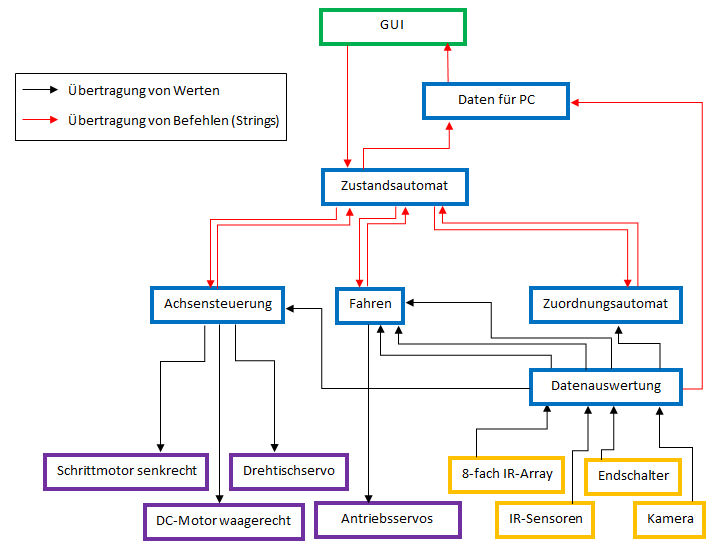
\includegraphics[width=\linewidth]{graphics/software_struktur.png}
\end{center}
\caption{Realisierte Software-Struktur in LABView}
\label{fig:software_struktur}
\end{figure}

\subsection{Unterkapitel}

Ein Beispiel für die Darstellung von Formeln. Aus den nachfolgenden zwei Formeln ist ersichtlich, dass sie das gleiche Verhältnis zwischen den Quadraten der drei Seiten eines rechtwinkligen Dreiecks darstellen, wobei $a$ und $b$ für die Längen der beiden Katheten und $c$ für die Länge der Hypotenuse steht. Aus dem Satz des Pythagoras,
\begin{equation}
a^2+b^2=c^2\;,
\end{equation}
lässt sich mit Hilfe einer einfachen Umformung das Quadrat der einen Kathete des rechtwinkligen Dreiecks aus den Quadraten der anderen beiden Seitenlän-gen herleiten:
\begin{equation}
a^2=c^2-b^2\;.
\end{equation}

Durch eine andere Umformung erhält man auch das Quadrat der anderen Kathete:
\begin{equation}
b^2=c^2-a^2\;.
\end{equation}

Wie die Formeln in Word korrekt zu formatieren und die Nummerierung am rechten Seitenrand zu platzieren sind, ist den Videos auf der PF-IK zu entnehmen. \LaTeX macht das automatisch für Sie.
